\documentclass[tikz]{standalone}
\usepackage[utf8x]{inputenc}
\usepackage{amsmath}
\usepackage{tikz}
\usetikzlibrary{arrows,positioning}
\begin{document}
    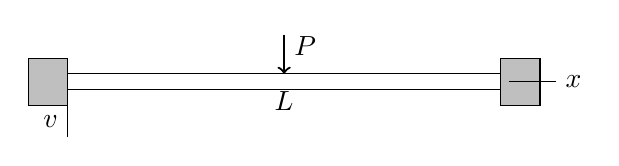
\begin{tikzpicture}
        \draw [fill=gray!50] (0, 0) rectangle (0.5, 0.6);
        \draw (0.5, 0.2) rectangle (6, 0.4) node [midway, below] {$L$}; 
        \draw [fill=gray!50] (6, 0) rectangle (6.5, 0.6);
        \draw [thick, ->] (3.25, 0.9) -- (3.25, 0.4) node [right, pos =0.3] {$P$};
        \draw (6.1, 0.3) -- (6.7, 0.3) node [right, pos= 1] {$x$};
        \draw (0.5, 0) -- (0.5, -0.4) node [left, pos=0.5] {$v$};
    \end{tikzpicture}
\end{document}